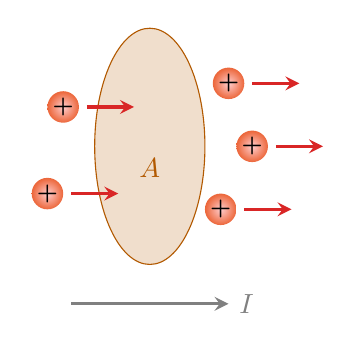
\begin{tikzpicture}[>=stealth]
  \draw[orange!70!black,fill=orange!70!black!20,name=conductor] (0,0) ellipse (0.7 and 1.5) node[below=0.8]{\(A\)};
  \draw[very thick,gray,->] (-1,-2) -- (1,-2) node[right]{\(I\)};

  \foreach \x\y in {-1.1/0.5,-1.3/-0.6,1/0.8,1.3/0,0.9/-0.8} {
    \shade[inner color=white!80!red, outer color=orange!50!red!70!lightgray] (\x,\y) node{\footnotesize\textbf{+}} circle (.2) [radius=1pt];
    \draw[very thick,color=red!70!gray,->] ({\x+0.3},\y) -- ({\x+0.9},\y);
  }

\end{tikzpicture}
